\documentclass[journal,12pt,twocolumn]{IEEEtran}
%\usepackage{chngcntr}
\usepackage{setspace}
\usepackage{float}
\usepackage{gensymb}
\singlespacing
% \usepackage[cmex10]{amsmath}
\usepackage{caption}
\usepackage{epstopdf}
\usepackage[cmex10]{amsmath}
\usepackage{amsthm}
%\interdisplaylinepenalty=2500
%\savesymbol{iint}
%\usepackage{txfonts}
%\restoresymbol{TXF}{iint}
%\usepackage{wasysym}
\usepackage{amsthm}
%\usepackage{iithtlc}
\usepackage{mathrsfs}
\usepackage{txfonts}
\usepackage[utf8]{inputenc}
\usepackage{float}
\usepackage{listings}
\usepackage{bm}
\usepackage{mathptmx}
\usepackage{amsfonts}
\usepackage{subfig}
\usepackage{xtab}
\usepackage{longtable}

%\usepackage{algorithm}
%\usepackage{algpseudocode}
%\usepackage{chngcntr}




\usepackage{mathrsfs}
\usepackage{txfonts}
\usepackage{stfloats}
\usepackage{bm}
\usepackage{cite}
% \usepackage{cases}
\usepackage{subfig}

\usepackage{longtable}
% \usepackage{multirow}

\usepackage{enumitem}
\usepackage{mathtools}
% \usepackage{steinmetz}
\usepackage{tikz}
%\usepackage{circuitikz}
\usepackage{verbatim}
% \usepackage{tfrupee}
\usepackage[breaklinks=true]{hyperref}
\usepackage{graphicx}
% \usepackage{tkz-euclide}

\usetikzlibrary{calc,math}
\usepackage{listings}
    \usepackage{color}                                            %%
    \usepackage{array}                                            %%
    \usepackage{longtable}                                        %%
    \usepackage{calc}                                             %%
    %\usepackage{multirow}                                         %%
    \usepackage{hhline}                                           %%
    \usepackage{ifthen}                                           %%
    \usepackage{lscape}     
\usepackage{multicol}
\usepackage{chngcntr}
\usepackage{xcolor}
%\DeclareMathOperator*{\Res}{Res}

\renewcommand\thesection{\arabic{section}}
\renewcommand\thesubsection{\thesection.\arabic{subsection}}
\renewcommand\thesubsubsection{\thesubsection.\arabic{subsubsection}}

\renewcommand\thesectiondis{\arabic{section}}
\renewcommand\thesubsectiondis{\thesectiondis.\arabic{subsection}}
\renewcommand\thesubsubsectiondis{\thesubsectiondis.\arabic{subsubsection}}


\hyphenation{op-tical net-works semi-conduc-tor}
\def\inputGnumericTable{}                                 %%

\lstset{
%language=C,
frame=single, 
breaklines=true,
columns=fullflexible
}
\begin{document}


\newtheorem{theorem}{Theorem}[section]
\newtheorem{problem}{Problem}
\newtheorem{proposition}{Proposition}[section]
\newtheorem{lemma}{Lemma}[section]
\newtheorem{corollary}[theorem]{Corollary}
\newtheorem{example}{Example}[section]
\newtheorem{definition}[problem]{Definition}

\newcommand{\BEQA}{\begin{eqnarray}}
\newcommand{\EEQA}{\end{eqnarray}}
\newcommand{\define}{\stackrel{\triangle}{=}}
\bibliographystyle{IEEEtran}
\raggedbottom
\setlength{\parindent}{0pt}
\providecommand{\mbf}{\mathbf}
\providecommand{\pr}[1]{\ensuremath{\Pr\left(#1\right)}}
\providecommand{\qfunc}[1]{\ensuremath{Q\left(#1\right)}}
\providecommand{\sbrak}[1]{\ensuremath{{}\left[#1\right]}}
\providecommand{\lsbrak}[1]{\ensuremath{{}\left[#1\right.}}
\providecommand{\rsbrak}[1]{\ensuremath{{}\left.#1\right]}}
\providecommand{\brak}[1]{\ensuremath{\left(#1\right)}}
\providecommand{\lbrak}[1]{\ensuremath{\left(#1\right.}}
\providecommand{\rbrak}[1]{\ensuremath{\left.#1\right)}}
\providecommand{\cbrak}[1]{\ensuremath{\left\{#1\right\}}}
\providecommand{\lcbrak}[1]{\ensuremath{\left\{#1\right.}}
\providecommand{\rcbrak}[1]{\ensuremath{\left.#1\right\}}}
\theoremstyle{remark}
\newtheorem{rem}{Remark}
\newcommand{\sgn}{\mathop{\mathrm{sgn}}}
\providecommand{\abs}[1]{\left\vert#1\right\vert}
\providecommand{\res}[1]{\Res\displaylimits_{#1}} 
\providecommand{\norm}[1]{\left\lVert#1\right\rVert}
%\providecommand{\norm}[1]{\lVert#1\rVert}
\providecommand{\mtx}[1]{\mathbf{#1}}
\providecommand{\mean}[1]{E\left[ #1 \right]}
\providecommand{\fourier}{\overset{\mathcal{F}}{ \rightleftharpoons}}
%\providecommand{\hilbert}{\overset{\mathcal{H}}{ \rightleftharpoons}}
\providecommand{\system}{\overset{\mathcal{H}}{ \longleftrightarrow}}
	%\newcommand{\solution}[2]{\textbf{Solution:}{#1}}
\newcommand{\solution}{\noindent \textbf{Solution: }}
\newcommand{\cosec}{\,\text{cosec}\,}
\providecommand{\dec}[2]{\ensuremath{\overset{#1}{\underset{#2}{\gtrless}}}}
\newcommand{\myvec}[1]{\ensuremath{\begin{pmatrix}#1\end{pmatrix}}}
\newcommand{\mydet}[1]{\ensuremath{\begin{vmatrix}#1\end{vmatrix}}}
%\numberwithin{equation}{subsection}

\makeatletter
\@addtoreset{figure}{problem}
\makeatother
\let\StandardTheFigure\thefigure
\let\vec\mathbf

\renewcommand{\thefigure}{\theproblem}

\def\putbox#1#2#3{\makebox[0in][l]{\makebox[#1][l]{}\raisebox{\baselineskip}[0in][0in]{\raisebox{#2}[0in][0in]{#3}}}}
     \def\rightbox#1{\makebox[0in][r]{#1}}
     \def\centbox#1{\makebox[0in]{#1}}
     \def\topbox#1{\raisebox{-\baselineskip}[0in][0in]{#1}}
     \def\midbox#1{\raisebox{-0.5\baselineskip}[0in][0in]{#1}}
\vspace{3cm}
\title{Assignment 1}
\author{Ishwari Prashad -EE18BTECH11020}
\maketitle
\newpage
\bigskip
\renewcommand{\thefigure}{\theenumi}
\renewcommand{\thetable}{\theenumi}



\section{Problem}
\begin{enumerate}[label=\thesection.\arabic*.,ref=\thesection.\theenumi]
    \numberwithin{equation}{enumi}
    
    \item Let
    \begin{align}
        x(n) = \cbrak{\underset{\uparrow}{1},2,3,4,2,1}
         \label{eq:equation0}\\
        y(n) + \frac{1}{2}y(n-1) = x(n) + x(n-2)	
        \label{eq:equation1}
    \end{align}
    
    \item Compute 
    \begin{align}
        X(k) \triangleq \sum_{n=0}^{N-1} x(n) e^{-j 2 \pi k n / N}, \quad k=0,1, \ldots, N-1
    \end{align}
    and $H(k)$ using h(n).
    
    \item Compute 
    \begin{align}
    Y(k) = X(k)H(k)
    \end{align}
\end{enumerate}

\section{Solution}
\begin{enumerate}[label=\thesection.\arabic*.,ref=\thesection.\theenumi]
\numberwithin{equation}{enumi}
\item
The Impulse Response of the LTI system is the output of the system when Unit Impulse Signal is given as input to the system.
Impulse response h(n) can be found from given difference equation as follows (h(n) is IIR Filter)
\begin{align}
    h(n) + \frac{1}{2}h(n-1) = \delta(n) + \delta(n-2)	
    \label{eq:equation4}
\end{align}

\item
DFT of a Input Signal $x(n)$ is 
\begin{align}
X(k) \triangleq \sum_{n=0}^{N-1} x(n) e^{-j 2 \pi k n / N}, \quad k=0,1, \ldots, N-1
\end{align}

\item
Let $W_{N} = e^{-j2\pi/N} \\$ 
We can express X as Matrix Multiplication of DFT Matrix and x.
\begin{equation}
X = 
\begin{bmatrix}
W^{ij}_{N} 
\end{bmatrix}_{N \times N}
x, \quad i,j = 0,1, \ldots, N-1
\end{equation}





\item
Using the Recursion property :
\begin{align}
	 W^{2}_{N} =  W_{N/2}  
\end{align}

\begin{align}
\mathcal X(k) &=  \sum_{n=0}^{N-1} x(n)W^{kn}_{N}, \quad k=0,1, \ldots, N-1 \\
&= \sum_{n=even} x(n)W^{kn}_{N} + \sum_{n=odd} x(n)W^{kn}_{N} \\
&= \sum_{m=0}^{2} x(2m)W^{2mk}_{N} + \sum_{m=0}^{2} x(2m+1)W^{(2m+1)k}_{N} 
\end{align}
using property above property, we get,
\begin{align}
\mathcal X(k) &= \sum_{m=0}^{2} x(2m)W^{mk}_{N/2} + W^{k}_{N} \sum_{m=0}^{2} x(2m+1)W^{mk}_{N/2} \\
&= X_{1}(k) + W^{k}_{N}X_{2}(k)
\end{align}

\begin{itemize}
	\item Here,X\textsubscript{1}(k) and X\textsubscript{2}(k) are 3 point DFTs of x(2m) and x(2m+1) , m=0,1,2.
	\item And X\textsubscript{1}(k) and X\textsubscript{2}(k) are periodic, Hence X\textsubscript{1}(k+3) = X\textsubscript{1}(k) and X\textsubscript{2}(k+3) = X\textsubscript{1}(k).
\end{itemize}
Taking N = 6 and expressing the even odd DFT's $X_{1}(k)$ , $X_{2}(k)$ interms of matrices we get,

\item
Let $F_{N}$ be the N-point DFT Matrix. \\
Using the property of Complex Exponentials we can express $F_{N}$ in terms of $F_{N/2}$
\begin{equation}
F_{N}=
\begin{bmatrix}
I_{N/2} & D_{N/2} \\
I_{N/2} & -D_{N/2}
\end{bmatrix}
\begin{bmatrix}
F_{N/2} & 0 \\
0 & F_{N/2}
\end{bmatrix}
P_{N}
\end{equation}
For N = 6
\begin{equation}
\implies F_{6}=
\begin{bmatrix}
I_{3} & D_{3} \\
I_{3} & -D_{3}
\end{bmatrix}
\begin{bmatrix}
F_{3} & 0 \\
0 & F_{3}
\end{bmatrix}
P_{6}
\end{equation}
where
$I_{3}$ is the 3x3 identity matrix. Writing some matrices in block form :
\begin{equation}
D_{3}=
\begin{bmatrix}
1 & 0 & 0 \\
0 & W^{1}_{3} & 0 \\
0 & 0 & W^{2}_{3}
\end{bmatrix}
\end{equation}
\begin{equation}
P_{6} =
\begin{bmatrix}
1 & 0 & 0 & 0 & 0 & 0\\
0 & 0 & 1 & 0 & 0 & 0\\
0 & 0 & 0 & 0 & 1 & 0\\
0 & 1 & 0 & 0 & 0 & 0\\
0 & 0 & 0 & 1 & 0 & 0\\
0 & 0 & 0 & 0 & 0 & 1
\end{bmatrix} 
\end{equation}
\begin{equation}
\implies P_{6}
\begin{bmatrix}
x(0) \\ 
x(1) \\ 
x(2) \\ 
x(3) \\ 
x(4) \\ 
x(5)
\end{bmatrix}
= 
\begin{bmatrix}
x(0) \\ 
x(2) \\ 
x(4) \\ 
x(1) \\ 
x(3) \\ 
x(5)
\end{bmatrix}
\end{equation}
Let 
\begin{equation}
\begin{bmatrix}
X_{1}(0) \\ 
X_{1}(1) \\ 
X_{1}(2) 
\end{bmatrix}
= F_{N/2}
\begin{bmatrix}
x(0) \\ 
x(2) \\ 
x(4) \\ 
\end{bmatrix}
\end{equation}
\begin{equation}
\begin{bmatrix}
X_{2}(0) \\ 
X_{2}(1) \\ 
X_{2}(2) 
\end{bmatrix}
= F_{N/2}
\begin{bmatrix}
x(1) \\ 
x(3) \\ 
x(5) \\ 
\end{bmatrix}
\end{equation}
be the N/2 point DFTs.
\item
By replacing the above results in the equation $X = F_{N} x$, we get
\begin{equation}
\begin{bmatrix}
X(0) \\ 
X(1) \\ 
X(2) \\ 
X(3) \\ 
X(4) \\ 
X(5) 
\end{bmatrix}
=
\begin{bmatrix}
1 & 0 & 0 & W^{0}_{6} & 0 & 0\\
0 & 1 & 0 &  0 & W^{1}_{6} & 0\\
0 & 0 & 1 & 0 & 0 & W^{2}_{6}\\
1 & 0 & 0 & -W^{0}_{6} & 0 & 0\\
0 & 1 & 0 & 0 & -W^{1}_{6} & 0\\
0 & 0 & 1 & 0 & 0 & -W^{2}_{6}
\end{bmatrix}
\begin{bmatrix}
X_{1}(0) \\ 
X_{1}(1)\\ 
X_{1}(2)\\ 
X_{2}(0) \\ 
X_{2}(1) \\ 
X_{2}(2)
\end{bmatrix}  
\end{equation}
Broke N-point DFT into 2 N/2-point DFTs using above method
\begin{equation}
\begin{bmatrix}
X(0) \\ 
X(1) \\ 
X(2) \\ 
\end{bmatrix}
=
\begin{bmatrix}
X_{1}(0) \\ 
X_{1}(1)\\ 
X_{1}(2)\\
\end{bmatrix}
+
\begin{bmatrix}
W^{0}_{6} & 0 & 0\\
0 & W^{1}_{6} & 0\\
0 & 0 & W^{2}_{6}\\
\end{bmatrix}
\begin{bmatrix}
X_{2}(0) \\ 
X_{2}(1) \\ 
X_{2}(2)
\end{bmatrix}
\end{equation}
\begin{equation}
\begin{bmatrix}
X(3) \\ 
X(4) \\ 
X(5) 
\end{bmatrix}
=
\begin{bmatrix}
X_{1}(0) \\  
X_{1}(1)\\ 
X_{1}(2)\\
\end{bmatrix}
-
\begin{bmatrix}
W^{0}_{6} & 0 & 0\\
0 & W^{1}_{6} & 0\\
0 & 0 & W^{2}_{6}\\
\end{bmatrix}
\begin{bmatrix}
X_{2}(0) \\ 
X_{2}(1) \\ 
X_{2}(2)
\end{bmatrix} 
\end{equation}
We can reduce our time complexity from O($N^{2}$) to O(NlogN) by doing this. 
\item Now, if $N = 2^{M}$ where $M \in \mathbb{Z^{+}}$  then we can recursively breakdown N/2 point DFT Matrix to N/4 point DFT Matrix ..so on till we reach 2-point DFT Matrix.So for N = 8, we can write,
\begin{equation}
F_{8}=
\begin{bmatrix}
I_{4} & D_{4} \\
I_{4} & -D_{4}
\end{bmatrix}
\begin{bmatrix}
F_{4} & 0 \\
0 & F_{4}
\end{bmatrix}
P_{8}
\end{equation}
\begin{equation}
F_{4}=
\begin{bmatrix}
I_{2} & D_{2} \\
I_{2} & -D_{2}
\end{bmatrix}
\begin{bmatrix}
F_{2} & 0 \\
0 & F_{2}
\end{bmatrix}
P_{4}
\end{equation}
Finally, the 2-point DFT Matrix is the base case 
\begin{equation}
F_{2}
\begin{bmatrix}
x_{1} \\
x_{2}
\end{bmatrix}
=
\begin{bmatrix}
1 & 1 \\
1 & -1
\end{bmatrix}
\begin{bmatrix}
x_{1} \\
x_{2}
\end{bmatrix}
=
\begin{bmatrix}
x_{1}+x_{2} \\
x_{1}-x_{2}
\end{bmatrix}
\end{equation}
\item Step by Step visualization of computing 8-Point DFT recursively using 4-point DFT's and 2-point DFT's.Expressing 8-point DFT's in terms of 4-point DFT's.
\begin{equation}
\begin{bmatrix}
X(0) \\ 
X(1) \\ 
X(2) \\ 
X(3)
\end{bmatrix}
=
\begin{bmatrix}
X_{e}(0) \\ 
X_{e}(1)\\ 
X_{e}(2)\\
X_{e}(3)\\
\end{bmatrix}
+
\begin{bmatrix}
W^{0}_{8} & 0 & 0 & 0\\
0 & W^{1}_{8} & 0 & 0\\
0 & 0 & W^{2}_{8} & 0\\
0 & 0 & 0 & W^{3}_{8}
\end{bmatrix}
\begin{bmatrix}
X_{o}(0) \\ 
X_{o}(1) \\ 
X_{o}(2) \\
X_{o}(3)
\end{bmatrix}
\end{equation}
\begin{equation}
\begin{bmatrix}
X(4) \\ 
X(5) \\ 
X(6) \\ 
X(7)
\end{bmatrix}
=
\begin{bmatrix}
X_{e}(0) \\ 
X_{e}(1)\\ 
X_{e}(2)\\
X_{e}(3)\\
\end{bmatrix}
-
\begin{bmatrix}
W^{0}_{8} & 0 & 0 & 0\\
0 & W^{1}_{8} & 0 & 0\\
0 & 0 & W^{2}_{8} & 0\\
0 & 0 & 0 & W^{3}_{8}
\end{bmatrix}
\begin{bmatrix}
X_{o}(0) \\ 
X_{o}(1) \\ 
X_{o}(2) \\
X_{o}(3)
\end{bmatrix}
\end{equation}
Now, 4-point DFT's to 2-point DFT's
\begin{equation}
\begin{bmatrix}
X_{e}(0) \\ 
X_{e}(1)\\ 
\end{bmatrix}
=
\begin{bmatrix}
X_{e_{1}}(0) \\ 
X_{e_{1}}(1)\\ 
\end{bmatrix}
+
\begin{bmatrix}
W^{0}_{4} & 0\\
0 & W^{1}_{4}
\end{bmatrix}
\begin{bmatrix}
X_{o_{1}}(0) \\ 
X_{o_{1}}(1) \\ 
\end{bmatrix}
\end{equation}
\begin{equation}
\begin{bmatrix}
X_{e}(2) \\ 
X_{e}(3)\\ 
\end{bmatrix}
=
\begin{bmatrix}
X_{e_{1}}(0) \\ 
X_{e_{1}}(1)\\ 
\end{bmatrix}
-
\begin{bmatrix}
W^{0}_{4} & 0\\
0 & W^{1}_{4}
\end{bmatrix}
\begin{bmatrix}
X_{o_{1}}(0) \\ 
X_{o_{1}}(1) \\ 
\end{bmatrix}
\end{equation}
\begin{equation}
\begin{bmatrix}
X_{o}(0) \\ 
X_{o}(1)\\ 
\end{bmatrix}
=
\begin{bmatrix}
X_{e_{2}}(0) \\ 
X_{e_{2}}(1)\\ 
\end{bmatrix}
+
\begin{bmatrix}
W^{0}_{4} & 0\\
0 & W^{1}_{4}
\end{bmatrix}
\begin{bmatrix}
X_{o_{2}}(0) \\ 
X_{o_{2}}(1) \\ 
\end{bmatrix}
\end{equation}
\begin{equation}
\begin{bmatrix}
X_{o}(2) \\ 
X_{o}(3)\\ 
\end{bmatrix}
=
\begin{bmatrix}
X_{e_{2}}(0) \\ 
X_{e_{2}}(1)\\ 
\end{bmatrix}
-
\begin{bmatrix}
W^{0}_{4} & 0\\
0 & W^{1}_{4}
\end{bmatrix}
\begin{bmatrix}
X_{o_{2}}(0) \\ 
X_{o_{2}}(1) \\ 
\end{bmatrix}
\end{equation}
\begin{equation}
P_{8}
\begin{bmatrix}
x(0) \\ 
x(1) \\ 
x(2) \\ 
x(3) \\ 
x(4) \\ 
x(5) \\
x(6) \\
x(7)
\end{bmatrix}
= 
\begin{bmatrix}
x(0) \\ 
x(2) \\ 
x(4) \\ 
x(6) \\
x(1) \\ 
x(3) \\ 
x(5) \\
x(7)
\end{bmatrix}
\end{equation}
\begin{equation}
P_{4}
\begin{bmatrix}
x(0) \\ 
x(2) \\ 
x(4) \\ 
x(6) \\
\end{bmatrix}
= 
\begin{bmatrix}
x(0) \\ 
x(4) \\ 
x(2) \\
x(6)
\end{bmatrix}
\end{equation}
\begin{equation}
P_{4}
\begin{bmatrix}
x(1) \\ 
x(3) \\ 
x(5) \\
x(7)
\end{bmatrix}
= 
\begin{bmatrix}
x(1) \\ 
x(5) \\ 
x(3) \\ 
x(7) \\
\end{bmatrix}
\end{equation}
Finally,
\begin{equation}
\begin{bmatrix}
X_{e_{1}}(0) \\ 
X_{e_{1}}(1)\\ 
\end{bmatrix}
= F_{2}
\begin{bmatrix}
x(0) \\ 
x(4) \\ 
\end{bmatrix}
=
\begin{bmatrix}
x(0)+x(4) \\ 
x(0)-x(4) \\ 
\end{bmatrix}
\end{equation}
\begin{equation}
\begin{bmatrix}
X_{o_{1}}(0) \\ 
X_{o_{1}}(1)\\ 
\end{bmatrix}
= F_{2}
\begin{bmatrix}
x(2) \\ 
x(6) \\ 
\end{bmatrix}
=
\begin{bmatrix}
x(2)+x(6) \\ 
x(2)-x(6) \\ 
\end{bmatrix}
\end{equation}
\begin{equation}
\begin{bmatrix}
X_{e_{2}}(0) \\ 
X_{e_{2}}(1)\\ 
\end{bmatrix}
= F_{2}
\begin{bmatrix}
x(1) \\ 
x(5) \\ 
\end{bmatrix}
=
\begin{bmatrix}
x(1)+x(5) \\ 
x(1)-x(5) \\ 
\end{bmatrix}
\end{equation}
\begin{equation}
\begin{bmatrix}
X_{o_{2}}(0) \\ 
X_{o_{2}}(1)\\ 
\end{bmatrix}
= F_{2}
\begin{bmatrix}
x(3) \\ 
x(7) \\ 
\end{bmatrix}
=
\begin{bmatrix}
x(3)+x(7) \\ 
x(3)-x(7) \\ 
\end{bmatrix}
\end{equation}
So, $X_{e_{2}} \in \text{DFT} \{x(1),x(5)\}$ and $X_{o_{2}} \in \text{DFT} \{x(3),x(7)\}$ would combine to give $X_{o}$ .
\\And $X_{e_{1}} \in \text{DFT} \{x(0),x(4)\}$ and $X_{o_{1}} \in \text{DFT} \{x(2),x(6)\}$ would combine to give $X_{e}$.
\item The following C program will compute and print the FFT (N-point where N is of the form $2^{n}$)
\begin{lstlisting}
https://github.com/ipsingh85/EE3025_IDP/tree/main/Assingment_1/codes/fft_algo.c
\end{lstlisting}
\item \emph{Time Complexity:}
Matrix multiplication of NxN matrix with Nx1 vector is there in DFT.
Hence it has $O(N^2)$ time complexity which is very slow for high $N$.
\newline
In this recursive approach which is termed as FFT - N-point FFT is broken down recursively into 2 N/2-point FFTs recursively.\\
Additionally $O(N)$ operation of Vector multiplication is performed on the N/2 point FFTs.
\begin{equation}
T(n) = 2T(n/2) + O(n)
\end{equation}
Solving this recurrence relation gives $O(NlogN)$ time complexity.
\item Computing $X(k)$, $H(k)$ and $Y(k)$ for 
\begin{align}
x(n) = \cbrak{\underset{\uparrow}{1},2,3,4,2,1,4,3}
\end{align}
with N = 8, using above FFT approach.
The following plots are obtained from the code given below:
\begin{figure}[!ht]
	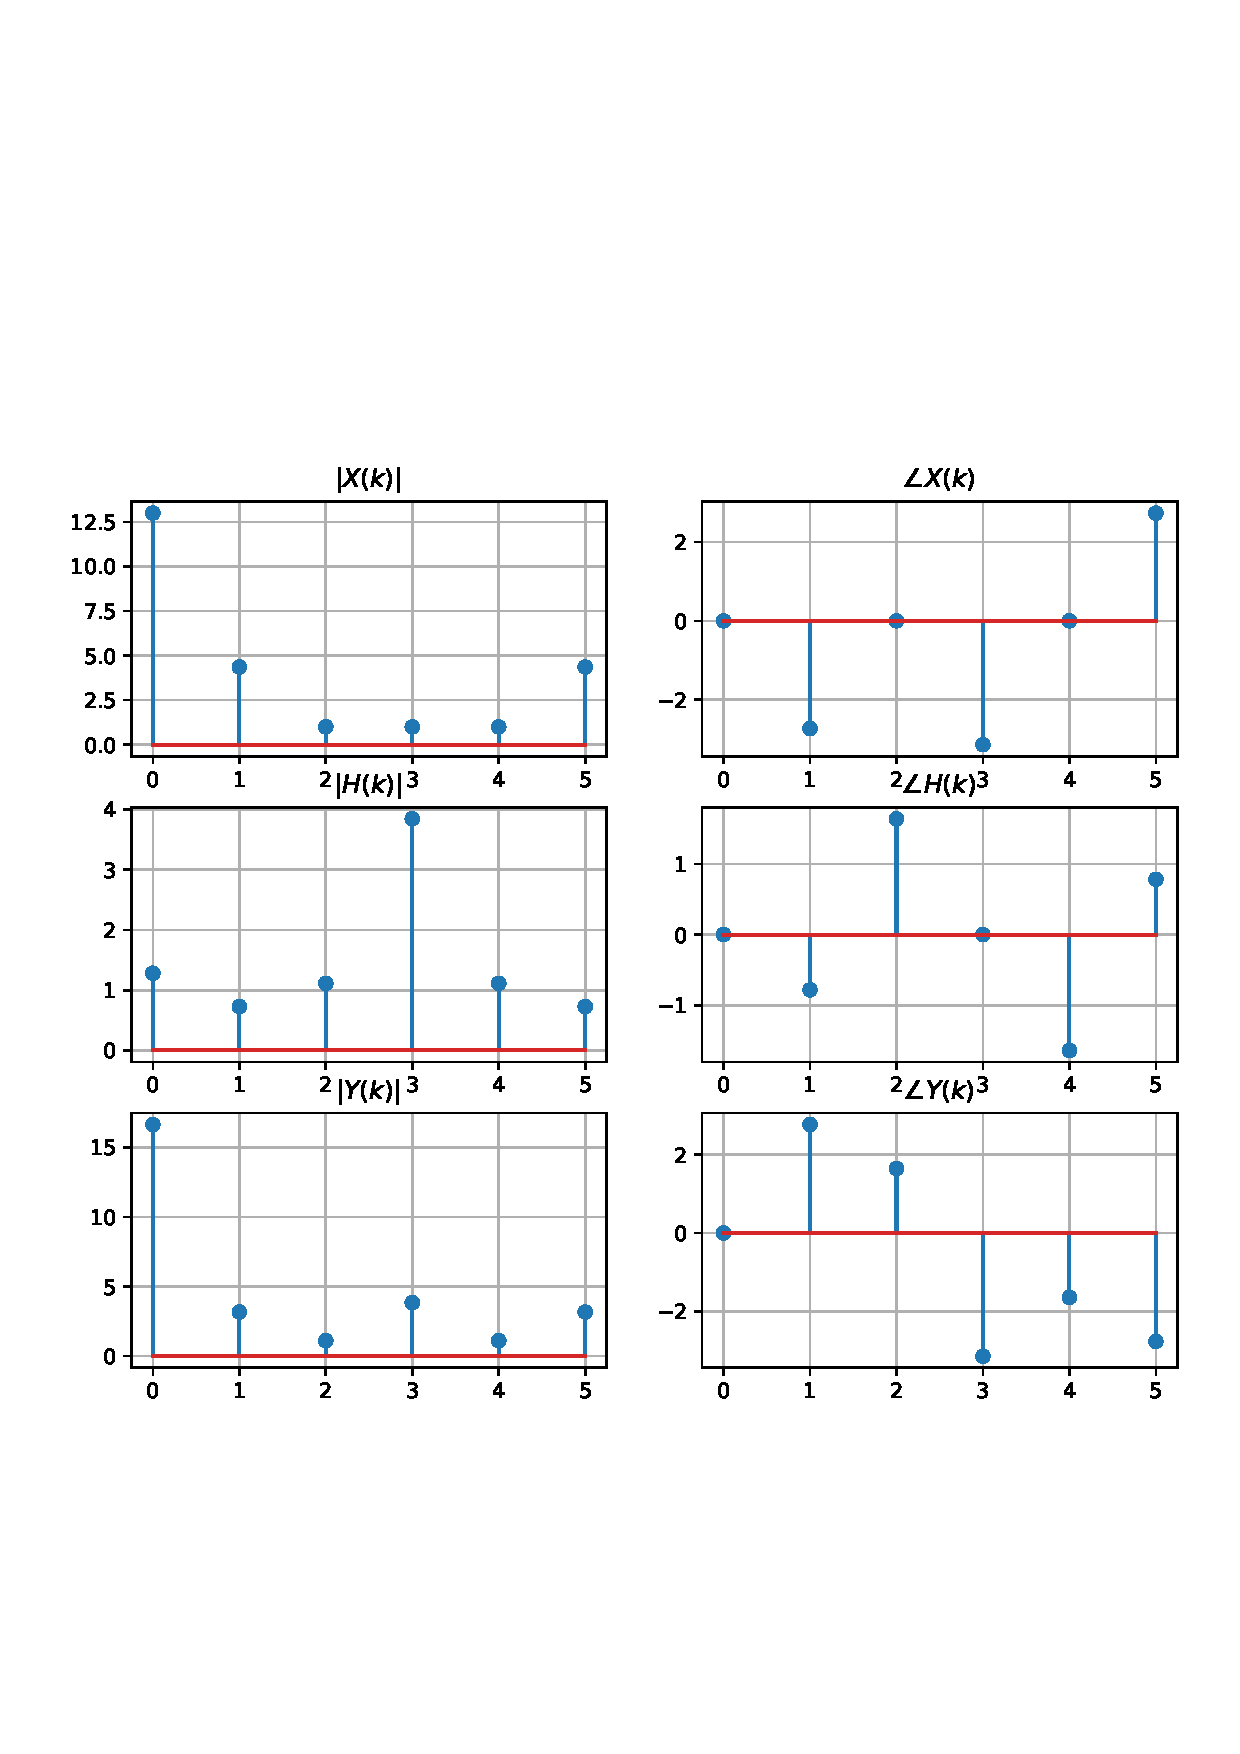
\includegraphics[width=1.15\columnwidth]{./figs/Figure_1.pdf}
\end{figure}
\\
\item This code plots above magnitude and phase plots of $X(k)$, $H(k)$ and $Y(k)$ .
\begin{lstlisting}
https://github.com/ipsingh85/EE3025_IDP/tree/main/Assingment_1/codes/ee18btech11020_1.py
\end{lstlisting}




\item \emph{Computation Times:} \\
We can compare the computation times for DFT,FFT and Inbuit-FFT algorithms for N = $2^{M}$, for N = 1 ($2^{0}$) to 8192 ($2^{13}$).
\item The below code plots the above time comparision plot.
\begin{lstlisting}
https://github.com/ipsingh85/EE3025_IDP/tree/main/Assingment_1/codes/ee18btech11020_2.py
\end{lstlisting}
\begin{figure}[!ht]
	\includegraphics[width=1.15\columnwidth]{./figs/Figure_2.pdf}
\end{figure}

\item Obtaining 8-Point FFT using DFT Matrix
\begin{equation}
\renewcommand{\arraystretch}{1.35}
\setlength\arraycolsep{0.05pt}
\begin{bmatrix}
X(0) \\
X(1) \\
X(2) \\
X(3) \\
X(4) \\
X(5) \\
X(6) \\
X(7)
\end{bmatrix}
=
\begin{bmatrix}
W^{0}_{8} & W^{0}_{8} & W^{0}_{8} & W^{0}_{8} & W^{0}_{8} & W^{0}_{8} & W^{0}_{8} & W^{0}_{8}\\
W^{0}_{8} & W^{1}_{8} & W^{2}_{8} & W^{3}_{8} & W^{4}_{8} & W^{5}_{8} & W^{6}_{8} & W^{7}_{8}\\
W^{0}_{8} & W^{2}_{8} & W^{4}_{8} & W^{6}_{8} & W^{8}_{8} & W^{10}_{8} & W^{12}_{8} & W^{14}_{8}\\
W^{0}_{8} & W^{3}_{8} & W^{6}_{8} & W^{9}_{8} & W^{12}_{8} & W^{15}_{8} & W^{18}_{8} & W^{21}_{8}\\
W^{0}_{8} & W^{4}_{8} & W^{8}_{8} & W^{12}_{8} & W^{16}_{8} & W^{20}_{8} & W^{24}_{8} & W^{28}_{8}\\
W^{0}_{8} & W^{5}_{8} & W^{10}_{8} & W^{15}_{8} & W^{20}_{8} & W^{25}_{8} & W^{30}_{8} & W^{35}_{8}\\
W^{0}_{8} & W^{6}_{8} & W^{12}_{8} & W^{18}_{8} & W^{24}_{8} & W^{30}_{8} & W^{36}_{8} & W^{42}_{8}\\
W^{0}_{8} & W^{7}_{8} & W^{14}_{8} & W^{21}_{8} & W^{28}_{8} & W^{35}_{8} & W^{42}_{8} & W^{49}_{8}
\end{bmatrix}
\begin{bmatrix}
1 \\
2 \\
3 \\
4 \\
2 \\
1 \\
0 \\
0
\end{bmatrix}
\end{equation}

\begin{equation}
\implies
\begin{bmatrix}
X(0) \\
X(1) \\
X(2) \\
X(3) \\
X(4) \\
X(5) \\
X(6) \\
X(7)
\end{bmatrix}
=
\begin{bmatrix}
13 \\
-3.121 - 6.535j \\
1j \\
1.121 - 0.535j \\
-1 \\
1.121 + 0.535j \\
-1j \\
-3.121 + 6.535j
\end{bmatrix}
\end{equation}
Similarly,

\begin{equation}
\begin{bmatrix}
H(0) \\
H(1) \\
H(2) \\
H(3) \\
H(4) \\
H(5) \\
H(6) \\
H(7)
\end{bmatrix}
=
\begin{bmatrix}
W^{0}_{8} & W^{0}_{8} & W^{0}_{8} & W^{0}_{8} & W^{0}_{8} & W^{0}_{8} & W^{0}_{8} & W^{0}_{8}\\
W^{0}_{8} & W^{1}_{8} & W^{2}_{8} & W^{3}_{8} & W^{4}_{8} & W^{5}_{8} & W^{6}_{8} & W^{7}_{8}\\
W^{0}_{8} & W^{2}_{8} & W^{4}_{8} & W^{6}_{8} & W^{8}_{8} & W^{10}_{8} & W^{12}_{8} & W^{14}_{8}\\
W^{0}_{8} & W^{3}_{8} & W^{6}_{8} & W^{9}_{8} & W^{12}_{8} & W^{15}_{8} & W^{18}_{8} & W^{21}_{8}\\
W^{0}_{8} & W^{4}_{8} & W^{8}_{8} & W^{12}_{8} & W^{16}_{8} & W^{20}_{8} & W^{24}_{8} & W^{28}_{8}\\
W^{0}_{8} & W^{5}_{8} & W^{10}_{8} & W^{15}_{8} & W^{20}_{8} & W^{25}_{8} & W^{30}_{8} & W^{35}_{8}\\
W^{0}_{8} & W^{6}_{8} & W^{12}_{8} & W^{18}_{8} & W^{24}_{8} & W^{30}_{8} & W^{36}_{8} & W^{42}_{8}\\
W^{0}_{8} & W^{7}_{8} & W^{14}_{8} & W^{21}_{8} & W^{28}_{8} & W^{35}_{8} & W^{42}_{8} & W^{49}_{8}
\end{bmatrix}
\begin{bmatrix}
1 \\
-0.5 \\
1.25 \\
-0.65 \\
0.3125 \\
-0.15625 \\
0.078125 \\
-0.0390625
\end{bmatrix}
\end{equation}

\begin{equation}
\implies
\begin{bmatrix}
H(0) \\
H(1) \\
H(2) \\
H(3) \\
H(4) \\
H(5) \\
H(6) \\
H(7)
\end{bmatrix}
=
\begin{bmatrix}
1.32 \\
0.858 - 0.514j \\
-0.015-0.007j \\
0.516 +1.829j \\
3.96 \\
0.516 - 1.829j \\
-0.015+0.007j  \\
0.858 + 0.514j
\end{bmatrix}
\end{equation}
So,
\begin{equation}
\begin{bmatrix} 
Y(0) \\ Y(1) \\ Y(2) \\ Y(3) \\ Y(4) \\ Y(5) \\ Y(6) \\ Y(7) 
\end{bmatrix}
=
\begin{bmatrix}
X(0)\cdot H(0) \\ X(1)\cdot H(1) \\ X(2)\cdot H(2) \\ X(3)\cdot H(3) \\ X(4)\cdot H(4) \\ X(5)\cdot H(5) \\ X(6)\cdot H(6) \\ X(7)\cdot H(7)
\end{bmatrix}
\end{equation}

\begin{equation}
\implies
\begin{bmatrix}
Y(0) \\
Y(1) \\
Y(2) \\
Y(3) \\
Y(4) \\
Y(5) \\
Y(6) \\
Y(7)
\end{bmatrix}
=
\begin{bmatrix}
17.16 \\
-6.04 - 4j \\
-0.007-0.015j \\
1.55 +1.77j \\
-3.96 \\
1.55 -1.77j\\
0.007+0.015j  \\
-6.04 + 4j
\end{bmatrix}
\end{equation}


\end{enumerate}
\end{document}